\documentclass[aspectratio=43]{beamer}

%%% Beamer options
\usetheme{Dresden}
\usecolortheme{beaver}
% remove the navigation buttons from the lower right
\beamertemplatenavigationsymbolsempty
% show slide numbers
\setbeamertemplate{footline}[frame number]

% error when symbols are not found in a font (since no font-fallback seems to exist)
% \tracinglostchars=3

\usepackage{amsmath}
\usepackage{amssymb}
\usepackage{amsfonts}
\usepackage{mathtools}
\usepackage{fontspec}
\usepackage{minted}
\usepackage{changepage}
\usepackage{todonotes}
\usepackage{newunicodechar}
\usepackage{graphicx}
\usepackage{mathpartir}

\setmonofont{Source Code Pro}
\newfontfamily\symfont{FreeMono}
\newfontfamily\symfontextra{FreeSerif}

% define some unicode characters missing from Source Code Pro
\newunicodechar{∗}{{\symfont ∗}}
\newunicodechar{⊥}{{\symfont ⊥}}
\newunicodechar{▷}{{\symfont ▷}}
\newunicodechar{↦}{{\symfont ↦}}
\newunicodechar{∨}{{\symfont ∨}}
\newunicodechar{∈}{{\symfont ∈}}
\newunicodechar{●}{{\symfont ●}}


% remove space for color box used in minted
\setlength{\fboxsep}{1pt}


\newcommand{\ocaml}[1]{\mintinline{ocaml}{#1}}
\newcommand{\coq}[1]{\mintinline{coq}{#1}}
\newcommand{\ocf}{OCaml~5}
\newcommand{\done}{{\symfontextra ✓}}
\newcommand{\tbd}{{\symfontextra ⌛}}
% \newcommand{\wand}{-\kern-.6em\raisebox{-.659ex}{*}\ }
\newcommand{\wand}{\mathrel{-\mkern-6mu*}}
\newcommand{\efork}{\ocaml{Fork}}
\newcommand{\esuspend}{\ocaml{Suspend}}
\newcommand{\egetctx}{\ocaml{GetContext}}
\newcommand{\proto}{\texttt{Coop}}
\newcommand{\ewp}[3]{\textit{ewp}\; (#1)\; \langle #2 \rangle\; \{#3\}}
\newcommand{\iriswp}[2]{\textit{wp}\; (#1)\; \{#2\}}
\newcommand{\pers}[1]{\Box\; #1}
\newcommand{\pinv}{\textit{promiseInv}}
\newcommand{\later}[1]{\triangleright\;#1}

\title{Verifying an Effect-Based Cooperative Concurrency Scheduler in Iris}
\author{Adrian Dapprich\\ Advisors: Prof. Derek Dreyer \& Prof. François Pottier}
\institute{Foundations of Programming Group, MPI-SWS, Saarland University}
\date{30. November 2023}

\begin{document}

\frame{\titlepage}

\section{Introduction}

% \begin{frame}{Self Introduction}
%     \begin{itemize}
%         \item Adrian Dapprich, master student and also former bachelor student at Saarland University.
%         \item Just finished an exchange year at Tohoku University at the lab of Prof. Sumii.
%         \item Interested in program verification, Rust \& embedded systems.
%     \end{itemize}
% \end{frame}

\begin{frame}{Today's Topic}
    \begin{itemize}
        \item Recently \ocf{} released with support for effect handlers.
        \item Eio is a multi-threaded, cooperative concurrency library for \ocf{} built around effects.
        \item Hazel\footnote{["Proof of Programs with Effect Handlers". Paulo de Vilhena. 2022]} is an implementation of a language with effect handlers in Iris.
        \item[\(\Rightarrow\)] We want to verify (a part of) the Eio library using Hazel to show the \textbf{safety} and \textbf{effect safety} of its central abstractions.
    \end{itemize}
\end{frame}

\begin{frame}{Why Eio?}
    \begin{itemize}
        \item Eio plans to replace previous concurrency libraries.
              \begin{itemize}
                  \item Effect handlers are more composable than monads, so easier to use than monadic-style concurrency libraries like \texttt{Lwt} and \texttt{Async}.
                  \item Effect handlers can be more efficient than monadic-style coding because it uses continuations for control flow instead of repeated bind operations.
              \end{itemize}
        \item There are already ports of multiple libraries to use Eio:
              \begin{itemize}
                  \item \texttt{SZXX}, \texttt{Irmin}, \texttt{ocaml-grpc}, \texttt{ocaml-cohttp}, OCaml CI solver service
                  \item More ports are being worked on.
              \end{itemize}
        \item[\(\Rightarrow\)] Verification of the core of a fundamental concurrency library in \ocf{} will provide a sense of safety for programmers using it.
    \end{itemize}
\end{frame}

\begin{frame}{Why Hazel?}
    \begin{itemize}
        \item Eio uses effects handlers for implementing cooperative concurrency.
        \item Eio uses the CQS\footnote{[Nikita Koval et al. 2023]. Already verified in Iris but Eio uses a customized variant which we want to verify.} lock-free datastructure for cross-thread communication.
        \item Hazel provides a framework for carrying out separation logic proofs about an ML-like language with effect handlers in Iris.
        \item[\(\Rightarrow\)] A perfect match!
    \end{itemize}

\end{frame}

\section{Background}

\begin{frame}[fragile]{Effect Handlers}
    \begin{itemize}
        \item Separate the code performing an effect from the code implementing an effect.
        \item Performing an effect captures the continuation up to the enclosing handler and jumps to the handler.
              \begin{itemize}
                  \item Also called "resumable exceptions"
                  \item A form of "delimited continuation" but easier to understand than \textit{shift/reset} etc.
              \end{itemize}
        \item \ocf{} supports effect handlers but without an effect system. Programs are not "effect-safe", i.e. there can be unhandled effects.
    \end{itemize}
\end{frame}


\begin{frame}[fragile]{Effect Handlers Example}
    % \begin{minted}[highlightlines={8},fontsize=\footnotesize]{ocaml}
    \begin{minted}[fontsize=\footnotesize]{ocaml}
type _ Effect.t += Get : unit -> int Effect.t
type _ Effect.t += Put : int -> unit Effect.t

let get () = perform (Get ())
let put v = perform (Put v)

let client () = 
  run ~init:0 (fun () ->
    for i = 0 to 5 do
      let x = get () in
      put (x + i)
    done;
    get ())

(* > client ();;
   => 15 *)
\end{minted}
\end{frame}

\begin{frame}[fragile]{Effect Handlers Example}
    % \begin{minted}[highlightlines={2,3,10,12},fontsize=\footnotesize]{ocaml}
    \begin{minted}[escapeinside=@@,fontsize=\footnotesize]{ocaml}
let run ~init f =
  let rec loop : @\colorbox{cyan}{\texttt{int -> (a, r) continuation -> a -> r}}@ =
    fun @\colorbox{cyan}{\texttt{state k x}}@ ->
      continue_with k x
      { retc = (fun result -> result);
        exnc = raise;
        effc = (fun (type b) (eff: b Effect.t) ->
          match eff with
          | Get () -> Some (fun (k: (b,r) continuation) ->
              @\colorbox{cyan}{\texttt{loop state k state}}@)
          | Put v -> Some (fun (k: (b,r) continuation) ->
              @\colorbox{cyan}{\texttt{loop v k ()}}@)
          | _ -> None)
      
  in
  loop init (fiber f) ()
\end{minted}
\end{frame}

\begin{frame}{Eio}
    \begin{itemize}
        \item Concurrency library for \ocf{} using the new effect handlers.
        \item Abstractions over OS resources like filesystem, network, etc.
        \item Synchronization constructs like mutexes, semaphores, etc.
              % \item Intends to be the main concurrency library for \ocf{}, replacing earlier \texttt{Async} and \texttt{Lwt}.
    \end{itemize}
\end{frame}


\begin{frame}{Eio (core)}
    \begin{columns}
        \begin{column}{0.5\textwidth}
            \begin{itemize}
                \item \ocaml{Fiber} represents a concurrent computation.
                \item \ocaml{Scheduler} runs \ocaml{Fiber}s in one thread and handles their effects.
                \item \ocaml{CQS} is used to implement synchronization constructs for multi-threading.
                \item \ocaml{Cancel} implements \ocaml{Fiber} cancellation.
                \item \ocaml{Switch} is used for scoped resource control.
            \end{itemize}
        \end{column}
        \begin{column}{0.5\textwidth}
            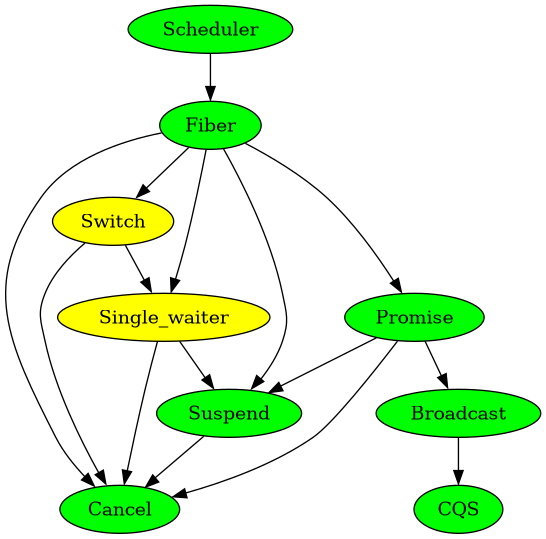
\includegraphics[width=\textwidth]{codept}
        \end{column}
    \end{columns}
\end{frame}

\begin{frame}{Hazel}
    \begin{itemize}
        \item Implementation of a language with effect handlers in Iris.
        \item Extended WP with protocols\footnote{Inspired by formalization of session types. The constructor can be read as: Performing the effect and passing value \(v\) satisfying \(P\), the effect handler will return a value \(w\) satisfying \(Q\).} that define which effects can be performed during evaluation.
        \item Existing case studies about control inversion \& cooperative concurrency.
        \item No multi-threading support and no atomic expressions defined.
        \item No type system but effect-safety is proved by extended WP.
    \end{itemize}
    \begin{align*}
        \text{Protocols:}   & \quad \Psi \Coloneqq \bot \mid\; !\; \vec{x}\; (v)\; \{ P \}.\; ?\; \vec{y}\; (w)\; \{ Q \} \mid ... \\
        \text{Extended WP:} & \quad \ewp{\texttt{e}}{\Psi}{w.\; Q}
    \end{align*}
\end{frame}

\section{Contribution}

\begin{frame}{Plan}
    Build an extended cooperative concurrency case study based on Eio using Hazel.
    \begin{itemize}
        \item The protocol \proto{} comprises three effects to communicate between fibers and their scheduler: \ocaml{Fork}, \ocaml{Suspend} \& \ocaml{GetContext}
              % \item Fibers can use OS resources
              % \item Fibers can be cancelled which signals them to stop and prevents OS resource usage.
        \item New threads can be forked which run a separate scheduler.
        \item Fibers can await other fibers (also cross-thread) using promises built on \ocaml{CQS}.
    \end{itemize}
    We do not plan to model switches as they are only used for resource cleanup.
    \begin{itemize}
        \item Fibers and resources are registered to switches. If all fibers have exited, the resources can be cleaned up.
        \item Switches are organized in a hierarchy and whole subtrees can be cancelled.
    \end{itemize}
\end{frame}

\begin{frame}{Plan}
    Build an extended cooperative concurrency case study based on Eio using Hazel.
    \begin{itemize}
        \item[\done{}] Simple cooperative concurrency scheduler using Eio effects, handling of promises in the fibers \& an axiomatization of CQS.
        \item[\done{}] Proof-of-concept for the \texttt{GetContext} effect.
        \item[\done{}] Definition of atomic expressions in Hazel.
        \item[\tbd{}] Add multi-threading to Hazel.
            \begin{itemize}
                \item[\tbd{}] Add support for the \texttt{iInv} tactic to Hazel.
            \end{itemize}
        \item[\done{}] Axiomatization of CQS is separately verified.
            \begin{itemize}
                \item[\tbd{}] When multi-threading primitives are added, port CQS development to Hazel and remove axioms.
            \end{itemize}
        \item[\tbd{}] Verify example client program that uses threads \& fibers.
    \end{itemize}
\end{frame}

\begin{frame}{Contribution}
    Let us look at an example interaction between the cooperative concurrency scheduler and a fiber performing an async computation.
    We focus on how a fiber awaits the completion of another fiber.
\end{frame}

\begin{frame}[fragile]{Client Fiber}
    Start two async network requests and wait for their completion (using the low-level API).
    \begin{minted}{ocaml}
let main () = 
    let p1 = fork_promise fetch_api in
    let p2 = fork_promise fetch_api in
    let r1 = await p1 in 
    let r2 = await p2 in 
    r1 + r2
    \end{minted}
    We assume
    \begin{align*}
         & \Phi \Coloneqq \lambda n. n \in \mathbb{N}                 \\
         & \ewp{\texttt{fetch\_api ()}}{\proto{}}{v. \pers{\Phi\; v}}
    \end{align*}
\end{frame}

\begin{frame}[fragile]{Fiber Operations}
    \ocaml{await} checks if promise is fulfilled and suspends if necessary, registering the waker.

    \begin{adjustwidth}{-2em}{0em}
        \begin{minipage}{0.45\textwidth}
            \begin{minted}[fontsize=\footnotesize]{ocaml}
let fork_promise f =
  let p = new_promise () in
  perform (Fork (fun () ->
    let v = f () in
    match !p with
    | Done _ -> assert false
    | Waiting cqs -> 
      p := Done v;
      Cqs.resume_all cqs
  ));
  p
\end{minted}
        \end{minipage}
        \begin{minipage}{0.5\textwidth}
            \begin{minted}[fontsize=\footnotesize]{ocaml}
let await p =
  match !p with
  | Done v -> v
  | Waiting cqs ->
    perform (Suspend (fun waker ->
      let req = Cqs.suspend cqs waker in
      match !p with
      | Done _ -> 
        if (Cqs.cancel cqs req)
        then waker ()
        else ()
      | Waiting _ -> ()
    ));
    match !p with
    | Done v -> v
    | Waiting _ -> assert false
\end{minted}
        \end{minipage}
    \end{adjustwidth}
\end{frame}


\begin{frame}[fragile]{Specifications}
    \ocaml{fork_promise} and \ocaml{await} form a pair where the promise returned from the first is used by the second.
    The specification of the scheduler \ocaml{run} shows that it handles all effects of its fibers.
    \begin{mathpar}
        %     promiseInv ∗ EWP (f #()) <| Coop  |> {{v, □ Φ v}}
        %   ⊢ 
        %     EWP (fork_promise f) <| Coop  |> {{ y, 
        %       ∃ (p: loc), ⌜ y = #p ⌝ ∗ isPromise p Φ }}.
        \inferrule [Fork]
        {\pinv{} \ast \ewp{\texttt{f ()}}{\proto{}}{v.\; \pers{\Phi\; v}}}
        {\ewp{\texttt{fork\_promise f}}{\proto{}}{p.\; \textit{isPromise}\; p\; \Phi}}
        % 
        \and
        % 
        % promiseInv ∗ isPromise p Φ ⊢ 
        %   EWP (await #p) <| Coop |> {{v, □ Φ v}}.
        \inferrule [Await]
        {\pinv{} \ast \textit{isPromise}\; p\; \Phi}
        {\ewp{\texttt{await p}}{\proto{}}{v.\; \pers{\Phi\; v}}}
        % 
        \and
        % 
        % promiseInv -∗
        %   (promiseInv -∗ EWP main #() <| Coop |> {{ v, □ Φ v }}) -∗
        %     EWP run main {{ _, True }}.
        \inferrule [Run]
        {\pinv{} \ast \ewp{\texttt{main ()}}{\proto{}}{\top}}
        {\ewp{\texttt{run main}}{\bot}{\top}}
    \end{mathpar}
\end{frame}

\begin{frame}[fragile]{Scheduler}
    \begin{minted}[fontsize=\footnotesize]{ocaml}
type 'a waker = 'a -> unit
type 'a suspender = 'a waker -> unit
type _ Effect.t += Fork : (unit -> unit) -> unit t
type _ Effect.t += Suspend : 'a suspender -> 'a t

let rec handle_fiber (e : unit -> unit) =
  match_with e () {
    effc = fun eff ->
      match eff with
      | Fork f -> Some (fun k ->
        Queue.add (fun () -> continue k ()) run_queue;
        handle_fiber f)
      | Suspend suspender -> Some (fun k -> 
        let waker = fun v -> 
          Queue.add (fun () -> continue k v) run_queue in
        suspender waker;
        next ());
    ...
   }
    \end{minted}
\end{frame}

\begin{frame}{Scheduler}
    \begin{itemize}
        \item The scheduler runs \ocaml{handle_fiber} for each fiber to handle their effects.
        \item The \ocaml{Fork} effect just runs \ocaml{handle_fiber} for the new fiber.
        \item The \ocaml{Suspend} effect carries a function that is called with a \ocaml{waker}, which is used to put the suspended fiber back into the run queue. Either immediately, or \ocaml{waker} is registered as a callback somewhere.
    \end{itemize}
\end{frame}

\begin{frame}{Execution Diagram}
    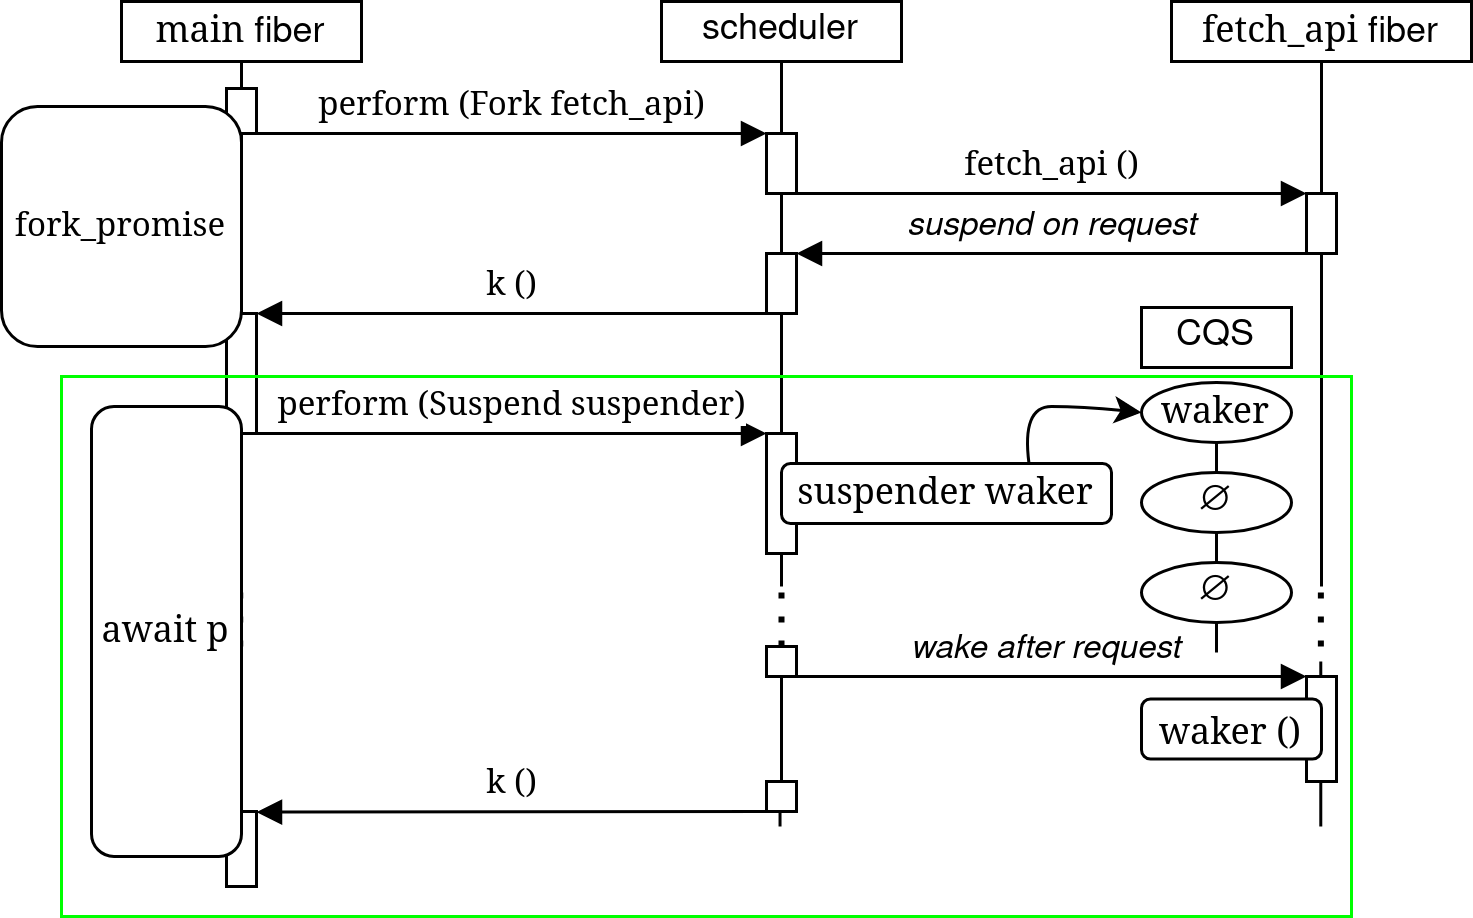
\includegraphics[width=\textwidth]{sequence diagram.png}
\end{frame}

\begin{frame}[fragile]{\ocaml{await} in Detail}
    \begin{adjustwidth}{-2em}{0em}
        \begin{minipage}{0.4\textwidth}
            \begin{itemize}
                \item 1st match checks if value can be returned immediately.
                \item 2nd match checks if fiber should really suspend.
                \item Must try to cancel in \ocaml{suspend} to ensure fiber is not lost.
                \item 3rd match knows that the promise is fullfilled after \ocaml{suspend} returns.
            \end{itemize}
        \end{minipage}
        \begin{minipage}{0.5\textwidth}
            \begin{minted}[escapeinside=@@,fontsize=\footnotesize]{ocaml}
let await p =
  @\colorbox{cyan}{\texttt{match !p with}}@
  | Done v -> v
  | Waiting cqs ->
    perform (Suspend (fun waker ->
      let req = Cqs.suspend cqs waker in
      @\colorbox{cyan}{\texttt{match !p with}}@
      | Done _ -> 
        @\colorbox{yellow}{\texttt{if (Cqs.cancel cqs req)}}@
        then waker ()
        else ()
      | Waiting _ -> ()
    ));
    @\colorbox{cyan}{\texttt{match !p with}}@
    | Done v -> v
    | Waiting _ -> @\colorbox{red}{\texttt{assert false}}@
\end{minted}
        \end{minipage}
    \end{adjustwidth}
\end{frame}

\begin{frame}[fragile]{Scheduler Ghost State}
    Promises are either waiting or already done.\newline
    %     \vspace{0.5em}
    \begin{minted}[fontsize=\footnotesize]{coq}
Definition promise_state_waiting γ := own γ (Cinl (1/2)%Qp).
Definition promise_state_done γ := own γ (Cinr (to_agree ())).
    \end{minted}
    Each \ocaml{waker} in a promise's queue represents a suspended fiber waiting for the result. So it may only be called with the knowledge that the promise is done.
    \begin{minted}[fontsize=\footnotesize]{coq}
Definition is_callback (P : iProp) (callback : val) := 
    P -∗ EWP (callback #()) {{_, True}}.
    \end{minted}
    Require \coq{is_callback (promise_state_done γ)} for CQS operations.
\end{frame}

\begin{frame}[fragile]{Scheduler Ghost State}
    To interact with promises from multiple threads we keep an authoritative map containing all promises in an invariant.
    Each promise is either done or waiting.
    \begin{itemize}
        \item[Done:] it contains a value satisfying a saved predicate \(\Phi\).
        \item[Waiting:] it contains a queue of suspended fibers.
    \end{itemize}
    \begin{minted}[fontsize=\footnotesize]{coq}
Definition promiseInv_inner : iProp := (
  ∃ M, own promise_name (● M) ∗ 
    [∗ map] args ↦ Φ ∈ M, let '(p, γ, ε) := args in
      (∃ y, p ↦ Done' y ∗ promise_state_done γ ∗ □ Φ y)
    ∨
      (∃ cqs, p ↦ Waiting' cqs ∗
        promise_state_waiting γ ∗
        (∃ n, thread_queue_state n) ∗
        resume_all_permit ∗
        is_cqs cqs)).
    \end{minted}
\end{frame}

\begin{frame}{A note on cancellation}
    \begin{itemize}
        \item Eio has a mechanism for cancelling fibers.
        \item We tried to define a suitable specification for cancelled fibers.
              \begin{itemize}
                  \item A cancelled fiber cannot use any OS resources.
                  \item So we verify that the history of OS resource usage of a fiber does not grow after cancellation.
              \end{itemize}
        \item But fibers can become "protected" and be free of the restrictions of cancellation.
        \item Fibers can even protect themselves after noticing they are cancelled.
        \item Therefore, cancellation is just a signalling mechanism without any enforcable and thus verifiable behavior.
    \end{itemize}
\end{frame}

\begin{frame}{CQS (CancellableQueueSynchronizer)}
    \begin{itemize}
        \item Lock-free queue to synchronize multiple threads.
              \begin{itemize}
                  \item \ocaml{suspend} operation inserts a callback.
                  \item \ocaml{cancel} operation removes a callback.
                  \item \ocaml{resume_all} operation calls all callbacks.
              \end{itemize}
              \vspace{0.5em}
              \begin{minipage}{0.45\textwidth}
                  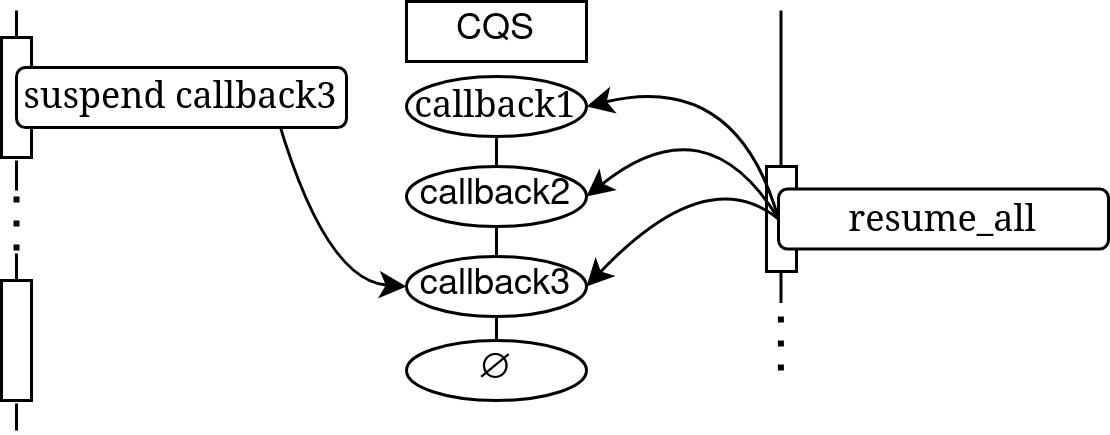
\includegraphics[width=\textwidth]{cqs-resume.png}
              \end{minipage}
              \begin{minipage}{0.45\textwidth}
                  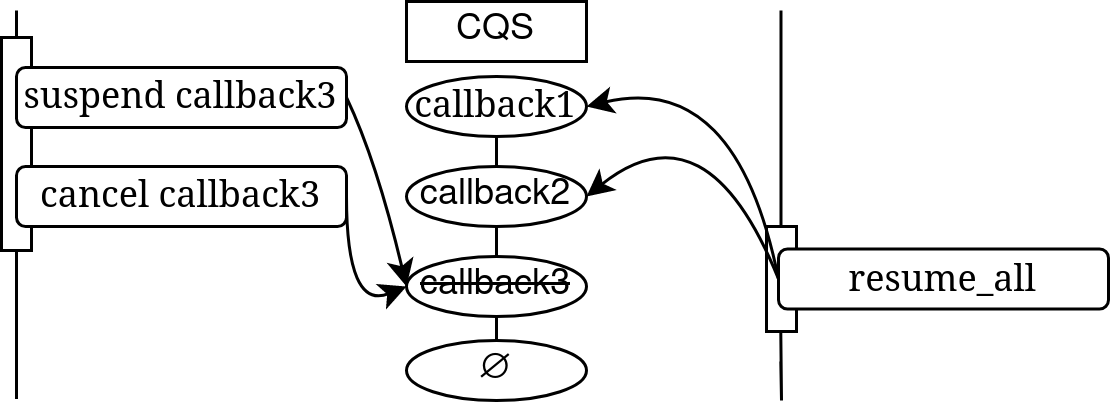
\includegraphics[width=\textwidth]{cqs-cancel.png}
              \end{minipage}
        \item Original CQS uses futures, we adapted the proof to callbacks.
        \item In Eio, the suspend callback places the fiber back in the run queue. So until it is called the fiber is blocked.\footnote{If a callback is missed by the queue, the fiber never runs again. Reasoning on paper shows that no callbacks are missed but to prove it in Iris we would need to use something like Iron [Bizjak et al. 2019]}
    \end{itemize}
\end{frame}

\begin{frame}[fragile]{CQS Logical State}
    \only<1>{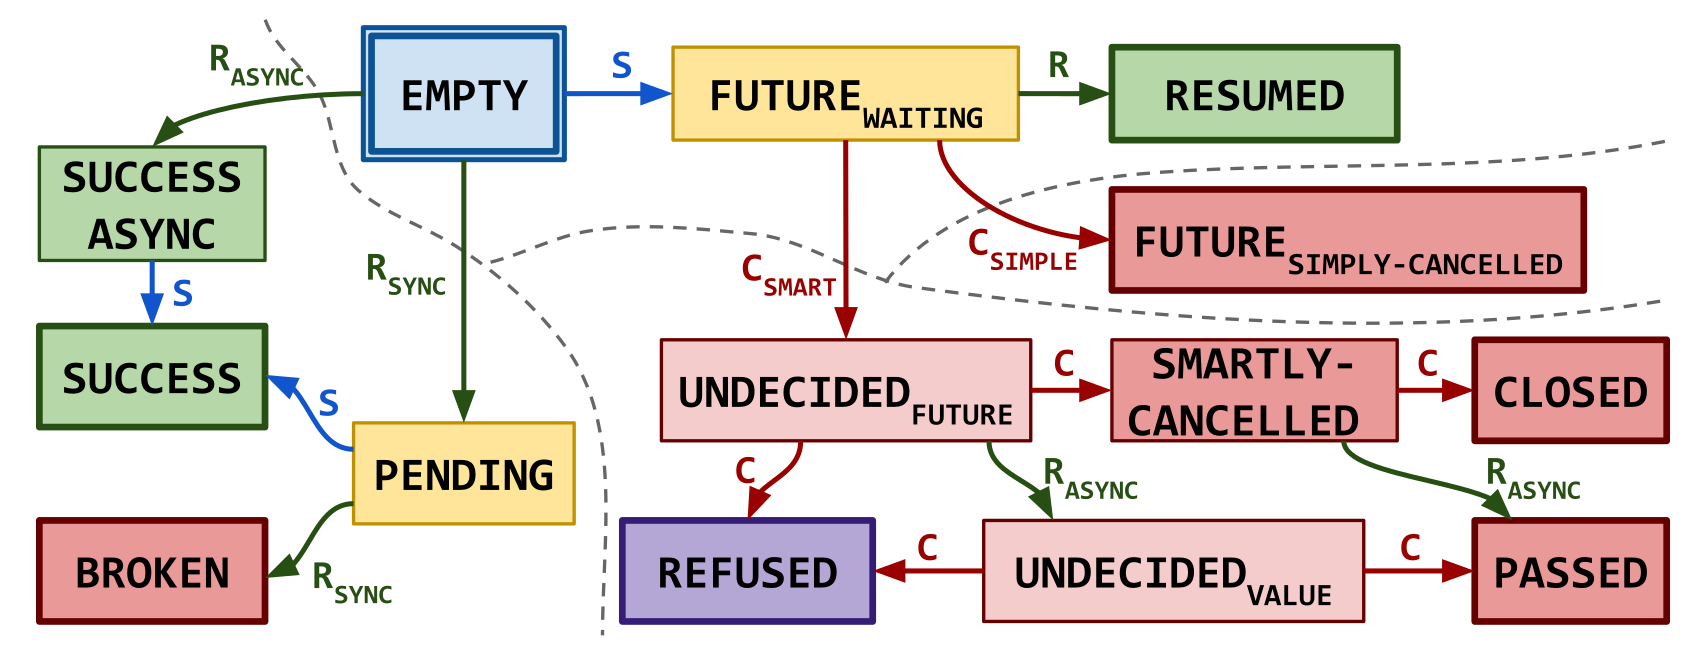
\includegraphics[width=\textwidth]{cqs-state-full.png}}
    \only<2>{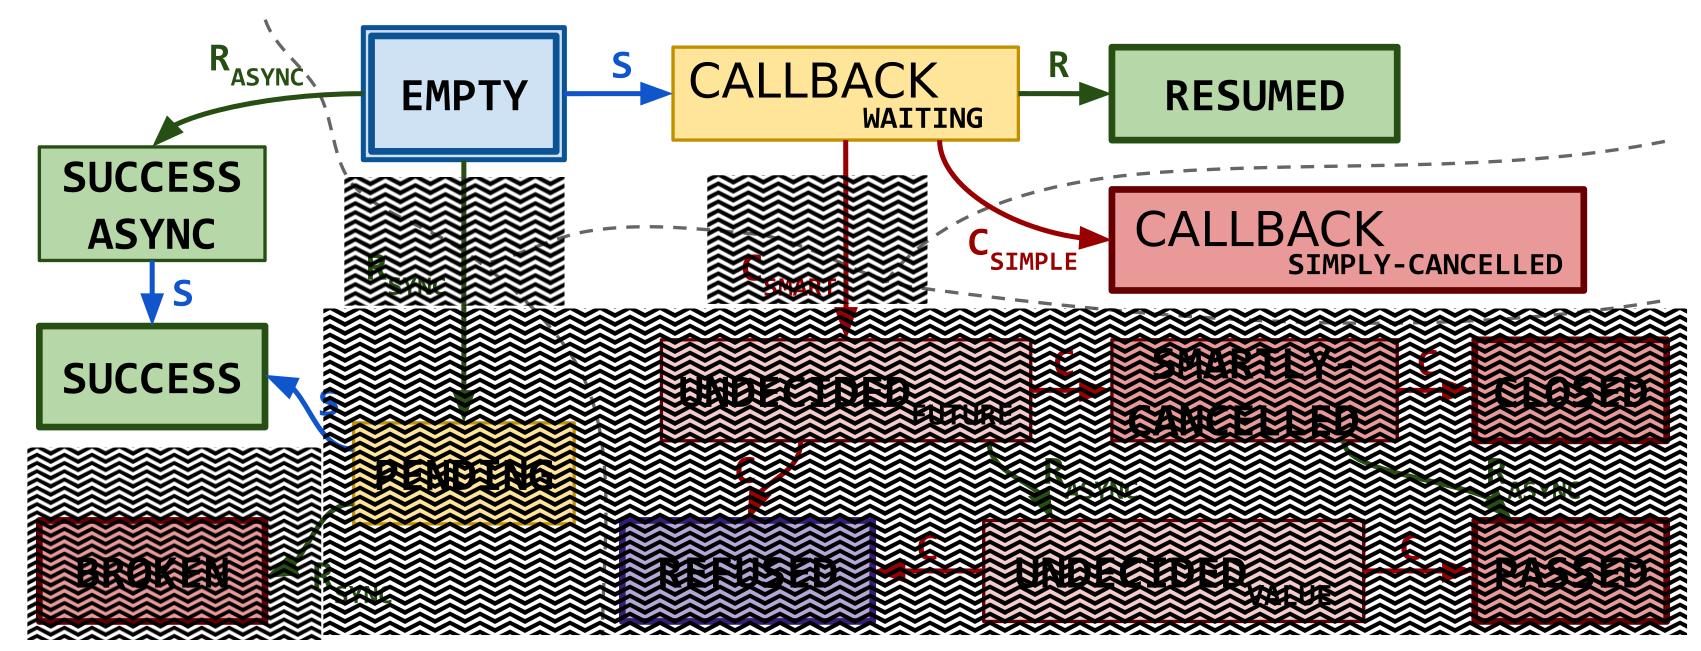
\includegraphics[width=\textwidth]{cqs-state-eio.png}}
\end{frame}

\begin{frame}{Multi-threading in Hazel}
    \begin{itemize}
        \item Same approach as WP, we track forked-off threads in EWP.
        \item Effects are not allowed to cross thread boundaries so a \ocaml{fork}\footnote{Better be careful about naming with regards to forking threads vs. fibers.} primitive needs to enforce the empty protocol.
        \item \coq{ewp_fork} \textit{should} follow by definition like in WP.
              \[
                  \inferrule [Fork]
                  {\ewp{\texttt{e}}{\bot}{\top}}
                  {\ewp{\texttt{fork e}}{\bot}{v. v = ()}}
              \]
        \item Adequacy of EWP \textit{should} still be provable by
              \[
                  \ewp{e}{\bot}{\Phi} \wand{} \iriswp{e}{\Phi}
              \]
    \end{itemize}
\end{frame}

\section{Conclusion}
\begin{frame}{Tentative Evaluation}
    \begin{itemize}
        \item Our case study shows that an Eio-like scheduler with \efork{}, \esuspend{} \& \egetctx{} effects is safe to use.
        \item We also have shown that it uses CQS correctly as a synchronization primitive.
        \item Eio has more ways of forking fibers and a hierarchy of cancellation contexts, which can be protected from cancellation. This part is not modelled.
    \end{itemize}
\end{frame}

\begin{frame}{Summary}
    \begin{itemize}
        \item We have finished a simple scheduler case study approximating Eio using the \efork{} \& \esuspend{} effects.
        \item Separately, we implemented a case study on the \egetctx{} effect to get meta-data about the current fiber.
        \item We have verified an adapted specification for Eio's custom CQS datastructure.
        \item Currently, we are working on adding multi-threading to Hazel.
    \end{itemize}
    Next, we want to extend the case study. This includes combining the above points, as well as:
    \begin{itemize}
        \item[\tbd{}] Add support for the \texttt{iInv} tactic to Hazel.
        \item[\tbd{}] Port CQS development to Hazel and remove axioms.
        \item[\tbd{}] Verify example client program that uses threads \& fibers.
    \end{itemize}
\end{frame}

\section{Misc}

\begin{frame}[fragile]{How \esuspend{} returns a proof that the promise is fulfilled}
    \begin{itemize}
        \item \(P\; v\) must be provided to call \ocaml{waker}.
        \item Waker registers the continuation of the effect to be invoked, so \(P\; v\) can be in the postcondition of the effect.
        \item In the case of \ocaml{await}, \(P \coloneqq \lambda \_. promise\_state\_done~\gamma\).
    \end{itemize}
    \begin{align*}
        \textit{isSuspender}\; f\; \Coloneqq & \; \forall \textit{waker}.\; \pinv{} \wand{}                                                                      \\
                                             & \quad (\forall v.\; P\; v \wand{} \textit{ewp}\; (\textit{waker}\; v)\; \langle \bot \rangle\; \{\top \}) \wand{} \\
                                             & \quad \triangleright \textit{ewp}\; (f\; waker)\; \langle \bot \rangle\; \{ \top \}                               \\
        \textit{SUSPEND}\;         \Coloneqq & \; !\; f\; P\; (f)\; \{ \pinv{} \ast \textit{isSuspender}\; f \}.                                                 \\
                                             & \;?\; v\; (v) \{ P\; v \}
    \end{align*}
\end{frame}

% \begin{frame}{Fiber-local storage}
%     \begin{itemize}
%         \item Eio supports fiber-local storage that can be queried by the \texttt{GetContext} effect.
%         \item Authoritative ghost map in the scheduler to save the storage \(\bullet [\texttt{gname} \mapsto (\bullet [\texttt{gname} \mapsto \textit{Val}])]\).
%         \item We parameterize the whole protocol by the ghost name of the storage of the current fiber.
%         \item That way both the scheduler and the fiber know which storage is accessible to the fiber.
%     \end{itemize}
% \end{frame}

\begin{frame}{Hazel Reasoning Rules}
    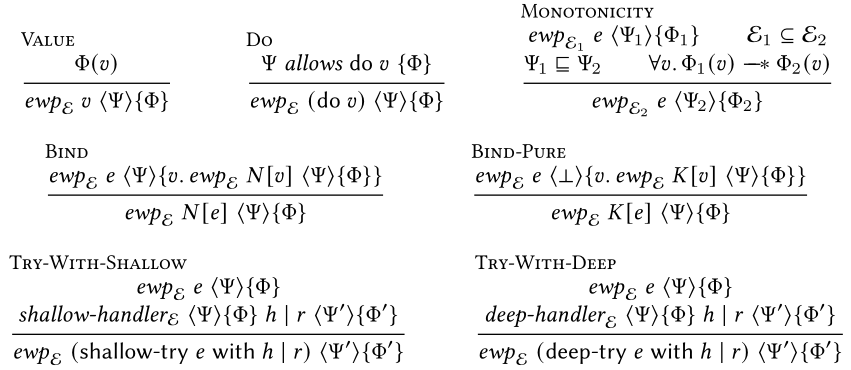
\includegraphics[width=\textwidth]{reasoning_rules1.png}
\end{frame}

\begin{frame}{Hazel Reasoning Rules}
    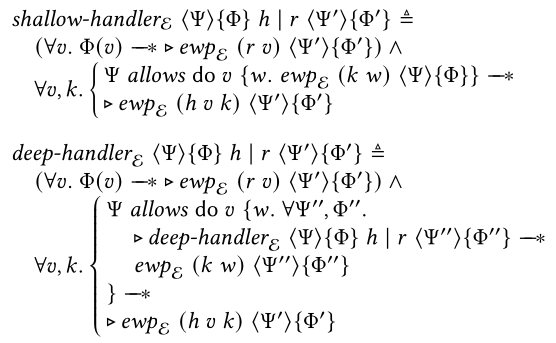
\includegraphics[width=\textwidth]{reasoning_rules2.png}
\end{frame}

% \begin{frame}{CQS API}
%     \begin{itemize}
%         \item CQS is a queue built on an infinite array of cells with two pointers into the array.
%         \item The \ocaml{suspend} \& \ocaml{resume} pointers are allowed to overtake each other.
%         \item \ocaml{suspend} creates a future and puts it into the next cell or immediately completes it if the cell is filled with a value.
%         \item \ocaml{resume} puts a value into the next cell or completes the future if the cell is filled with a future.
%         \item \ocaml{cancel} cancels the future from a cell.
%     \end{itemize}
% \end{frame}

% \begin{frame}{Customized CQS API}
%     \begin{itemize}
%         \item \ocaml{suspend} receives a callback instead of creating a future itself.\newline
%               \mintinline[fontsize=\footnotesize]{ocaml}{val suspend : t -> (unit -> unit) -> request option}
%         \item \ocaml{resume_all} resumes all callbacks with the same unit value.\newline
%               \mintinline[fontsize=\footnotesize]{ocaml}{resume_all : t -> unit}
%         \item \ocaml{cancel} is the same.
%     \end{itemize}
% \end{frame}

\end{document}